\documentclass[Lau, italian, noexaminfo]{sapthesis}

\usepackage[italian]{babel} %italian language package
\usepackage{epigraph} %quoting package
\usepackage{biblatex} %biblatex package, bibliography
\usepackage[utf8]{inputenc}
\usepackage{csquotes}
\usepackage{hyperref}
\usepackage{url}
\usepackage{graphicx} %graphics package
\usepackage{wrapfig} %for wrapping image and let text flanking image
\usepackage{subcaption} %for flanking images
\usepackage{minted} %for code snippets
\usemintedstyle{tango} %for coloring the code
\renewcommand\listoflistingscaption{Codici sorgente}
\renewcommand{\listingscaption}{Codice sorgente}
\usepackage[export]{adjustbox}
\usepackage{listings}
\usepackage{color}



\definecolor{dkgreen}{rgb}{0,0.6,0}
\definecolor{gray}{rgb}{0.5,0.5,0.5}
\definecolor{mauve}{rgb}{0.58,0,0.82}

\lstset{frame=tb,
  language=Go,
  aboveskip=3mm,
  belowskip=3mm,
  showstringspaces=false,
  columns=flexible,
  basicstyle={\small\ttfamily},
  numbers=none,
  numberstyle=\tiny\color{gray},
  keywordstyle=\color{blue},
  commentstyle=\color{dkgreen},
  stringstyle=\color{mauve},
  breaklines=true,
  breakatwhitespace=true,
  tabsize=3
}

%sapthesis class configuration
\title{Design ed Implementazione del Back End del  Sistema di Warehouse di SeismoCloud}
\author{Andrea Stella}
\IDnumber{1869065}
\course{Informatica}
\courseorganizer{Facoltà di Ingegneria dell'informazione, informatica e statistica}
\AcademicYear{2020/2021}
\copyyear{2021}
\advisor{Prof. Emanuele Panizzi}
\authoremail{stella.1869065@studenti.uniroma1.it}

%adding bibliography file
\addbibresource{bib/bibliography.bib}

\begin{document}

\maketitle

\frontmatter
\begin{abstract}

L'argomento della relazione di tirocinio verte sul design e sull'implementazione del lato Back End del Sistema di Warehouse dell'applicazione SeismoCloud. La relazione è suddivisa in cinque capitoli: il primo capitolo funge da \textbf{Introduzione} al progetto SeismoCloud ed alla relativa applicazione, mostrando un accenno dell'organizzazione del team di sviluppo dietro ad esso; nel secondo capitolo, \textbf{Analisi del problema}, si discutono le motivazioni alla base della creazione del Sistema di Warehouse, ovvero le problematiche che esso propone di risolvere; in \textbf{Design} si tratta la progettazione del sistema in sé e, in modo approfondito, del lato interno per la gestione delle richieste; nel capitolo di \textbf{Implementazione} sono invece mostrate le funzionalità sviluppate nel linguaggio Go, assieme ad alcune ottimizzazioni pensate per rendere il sistema più solido; infine, nel capitolo \textbf{Conclusione}, si riassume il lavoro compiuto, con una particolare attenzione agli sviluppi che possono derivare da esso.
    
    
    
    
\end{abstract}

\tableofcontents


\mainmatter
\chapter{Introduzione}

Il tirocinio è stato svolto all'interno del progetto \textbf{SeismoCloud}.\\
Di seguito viene innanzitutto introdotto il progetto stesso, mostrandone la struttura, lo scopo ed una visione ad alto livello del funzionamento delle sue componenti. Si trattano poi l'inserimento all'interno del team di sviluppo e gli strumenti utilizzati per tutta la durata del tirocinio.


\section{SeismoCloud, Earthquake Early Warning system}

\begin{wrapfigure}{r}{0.25\textwidth}
    \centering
    
\includegraphics[scale=0.15]{images/seismologo.png}
    \caption{Logo di SeismoCloud}
    \label{fig:seismologo}
\end{wrapfigure}

SeismoCloud \cite{seismocloud} è un progetto nato nel grazie al connubio dell'Università degli Studi di Roma “La Sapienza” e l’Istituto Nazionale di Geofisica e Vulcanologia (INGV). L'idea alla base del progetto è la rilevazione in tempo reale di scosse sismiche mediante una rete di sensori a basso costo e la segnalazione di un imminente terremoto alla popolazione della zona colpita tramite un'applicazione per dispositivi mobile. Il nome di quest'ultima ricalca il nome del progetto: \textit{SeismoCloud} (il logo è riportato nella Figura \ref{fig:seismologo}). Un sistema con queste finalità prende il nome di \textit{Earthquake Early Warning} (EEW).\\
\\
I dispositivi utilizzati per rilevare le scosse sismiche (da qui in avanti nominati \textit{Sismometri}) hanno un grande vantaggio che ne permette la rapida e semplice diffusione: il prezzo contenuto. Questa caratteristica consente alla rete di Sismometri di espandersi per sopperire all'unico svantaggio che si contrappone al modico prezzo: la precisione. Difatti, le rilevazioni di un singolo sismometro sono altamente imprecise, rendendo comuni vibrazioni (provocate, ad esempio, dal passaggio di una persona sulla stessa superficie su cui è posto il sismometro) un potenziale allarme. La costituzione di una fitta rete di Sismometri è essenziale per rendere il sistema completamente operativo ed affidabile nell'invio delle segnalazioni agli utenti dell'applicazione, motivo per cui, attualmente, la funzione di notifica preventiva non è ancora attiva.

\paragraph{I Sismometri}
I Sismometri sono i più validi alleati per la rilevazione delle scosse sismiche. La componente responsabile della misurazione delle vibrazioni prende il nome di \textbf{accelerometro}. Esso ne misura il valore basandosi sulla variazione di accelerazione che le scosse provocano su di ad esso.\\
L'accelerometro in sé, tuttavia, non ha una vera utilità se non viene collegato ad un dispositivo che lo gestisce e che invia i dati raccolti tramite Internet a SeismoCloud. Le alternative spaziano tra l'utilizzo di Raspberry Pi \cite{rpi} e di NodeMCU \cite{nodemcu}, dispositivi tipici dell'IoT, oltre che i dispositivi mobile stessi, dotati di un accelerometro. Sul sito web ufficiale di SeismoCloud \cite{seismocloud} è possibile trovare precise istruzioni su come creare il proprio sismometro con le componenti di cui sopra; inoltre, il codice per la loro configurazione è Open Source, disponibile sul profilo GitHub del progetto \cite{seismogit}. \\
La Figura \ref{fig:seismometers} mostra i Sismometri attivi sul territorio nazionale.

\begin{figure}[h!]
    \centering
    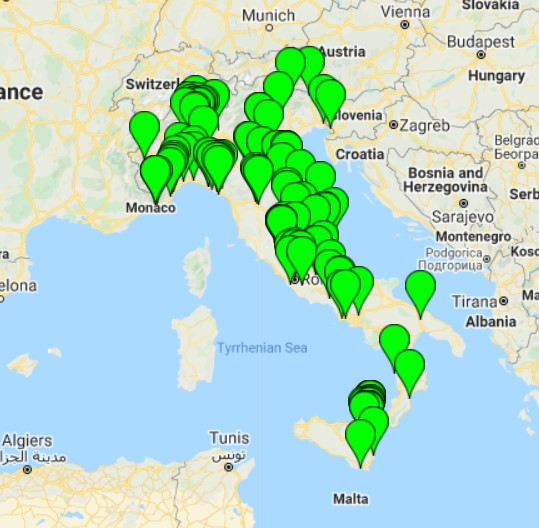
\includegraphics[width=\textwidth]{images/seismometersjpg.jpg}
    \caption{Sismometri attivi a livello nazionale}
    \label{fig:seismometers}
\end{figure}

\paragraph{Come si identifica un terremoto}
Si è discusso di quali sono gli elementi principali per la rilevazione delle scosse. Essi non sono però responsabili in maniera diretta della decisione da prendere sulla natura della scossa: questa decisione viene delegata al server che riceve i dati dei Sismometri. Grazie a degli algoritmi dedicati al processing delle informazioni sulle scosse in input, il server calcola se la vibrazione in cui sono incorsi i Sismometri è riconducibile ad una scossa sismica, e, a quel punto, aziona il meccanismo di Early Warning. 

\paragraph{La segnalazione}
Il sistema di EEW ha la capacità di salvare secondi preziosissimi agli utenti in caso di scossa sismica: si parla, difatti, di un avvertimento dai \textbf{2} ai \textbf{20} \textbf{secondi} prima dell'avvenimento del terremoto nel luogo in cui ci si trova, tempo utile non a fuggire ma a cercare riparo ed avere salva la vita.
A livello tecnico, la segnalazione di una scossa avviene tramite l'applicazione, che scatena la vibrazione tipica del ricevimento di una notifica sul dispositivo mobile. Vista l'importanza che questa notifica ha in caso di effettivo terremoto , la vibrazione può essere personalizzabile; inoltre, nei dispositivi Android, è possibile consentire all'applicazione di far vibrare il telefono anche se in modalità "silenziosa".

\paragraph{L'applicazione}

L'applicazione SeismoCloud, mostrata nella Figura \ref{fig:application}, rappresenta il punto di accesso a tutte le funzionalità offerte, come il monitoraggio dei propri Sismometri (Bottone \textit{Seismo} nella navigation bar), la visualizzazione del proprio profilo e delle impostazioni dell'applicazione (bottone \textit{Settings}), dei terremoti o delle scosse rilevate recentemente (bottone \textit{Quakes}, la schermata su cui ci si trova nell'immagine mostrata), dei gruppi di cui si è parte (bottone \textit{Groups}) e dei sensori presenti su una mappa (bottone \textit{Map}). 
Una delle funzioni fondamentali è raggiungibile cliccando su uno dei terremoti presenti nella lista (riportata in Figura \ref{fig:applicationsurvey}): oltre a presentare dei dati fondamentali relativi al terremoto (come l'istante di rilevamento, la sua posizione tramite visualizzazione sulla mappa, la distanza dalla posizione attuale del dispositivo attuale, la magnitudo del terremoto ed altre informazioni), l'applicazione permette agli utenti di rispondere ad un sondaggio in cui si chiedono dettagli su dove ci si trovasse, su cosa si facesse e su cosa si è percepito al momento del terremoto. Altre caratteristiche importanti sono accessibili tramite il bottone \textit{Settings}: è difatti possibile personalizzare la ricezione di una notifica in caso di Early Warning anche se in modalità silenziosa, attivare o disattivare la rilevazione tramite il sensore del dispositivo mobile e stabilire il consumo energetico massimo che l'applicazione attiva comporta (per approfondire quest'ultimo punto, consultare il lavoro di Enrico Bassetti \cite{enricobassetti}).

\begin{figure}[h]

\begin{subfigure}{0.5\textwidth}
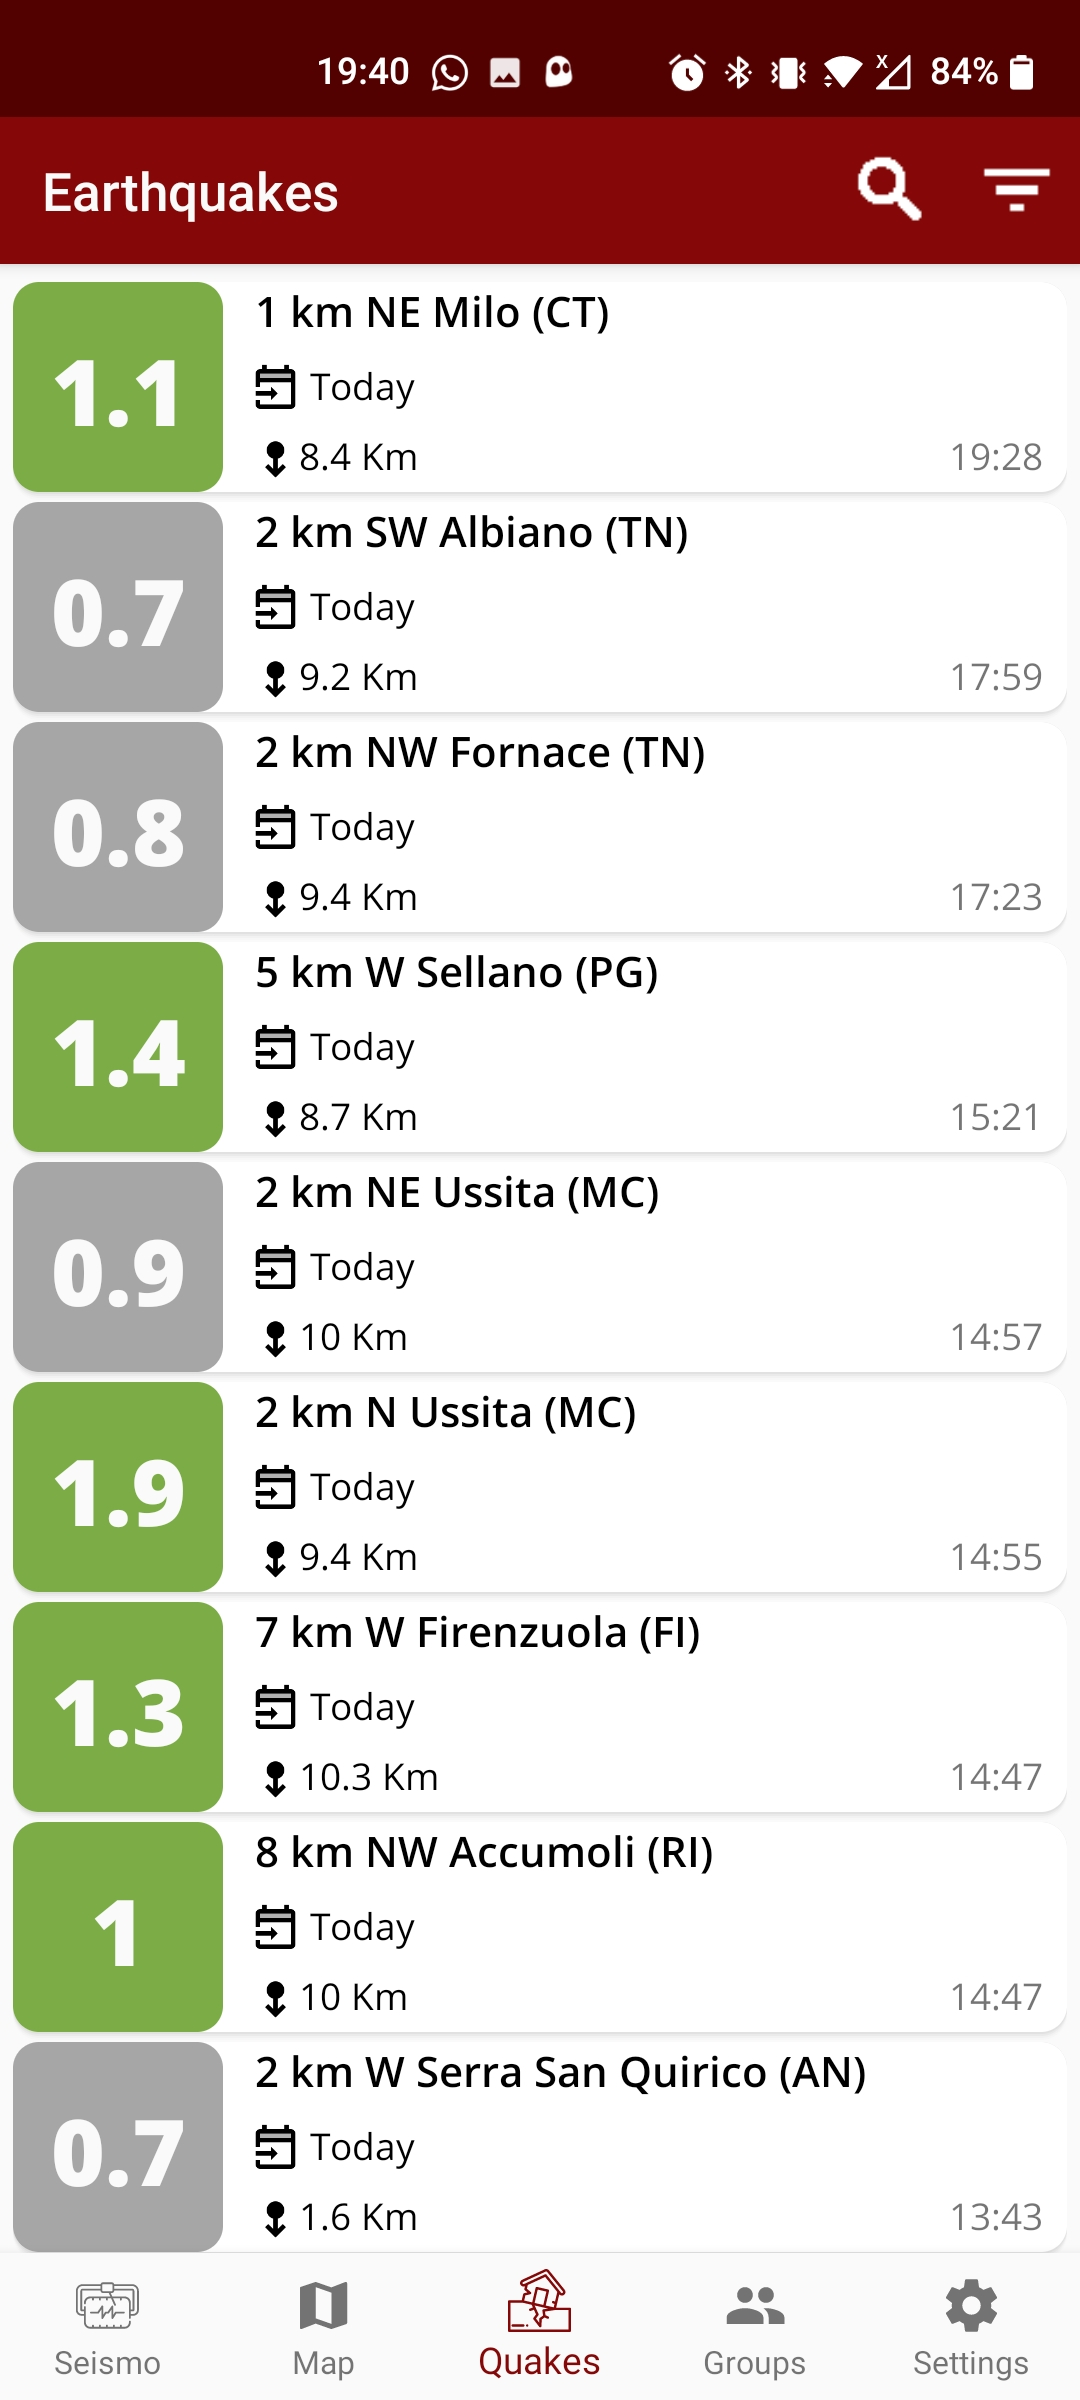
\includegraphics[width=0.9\linewidth]{images/application.png} 
\caption{Schermata dei terremoti}
\label{fig:application}
\end{subfigure}
\begin{subfigure}{0.5\textwidth}
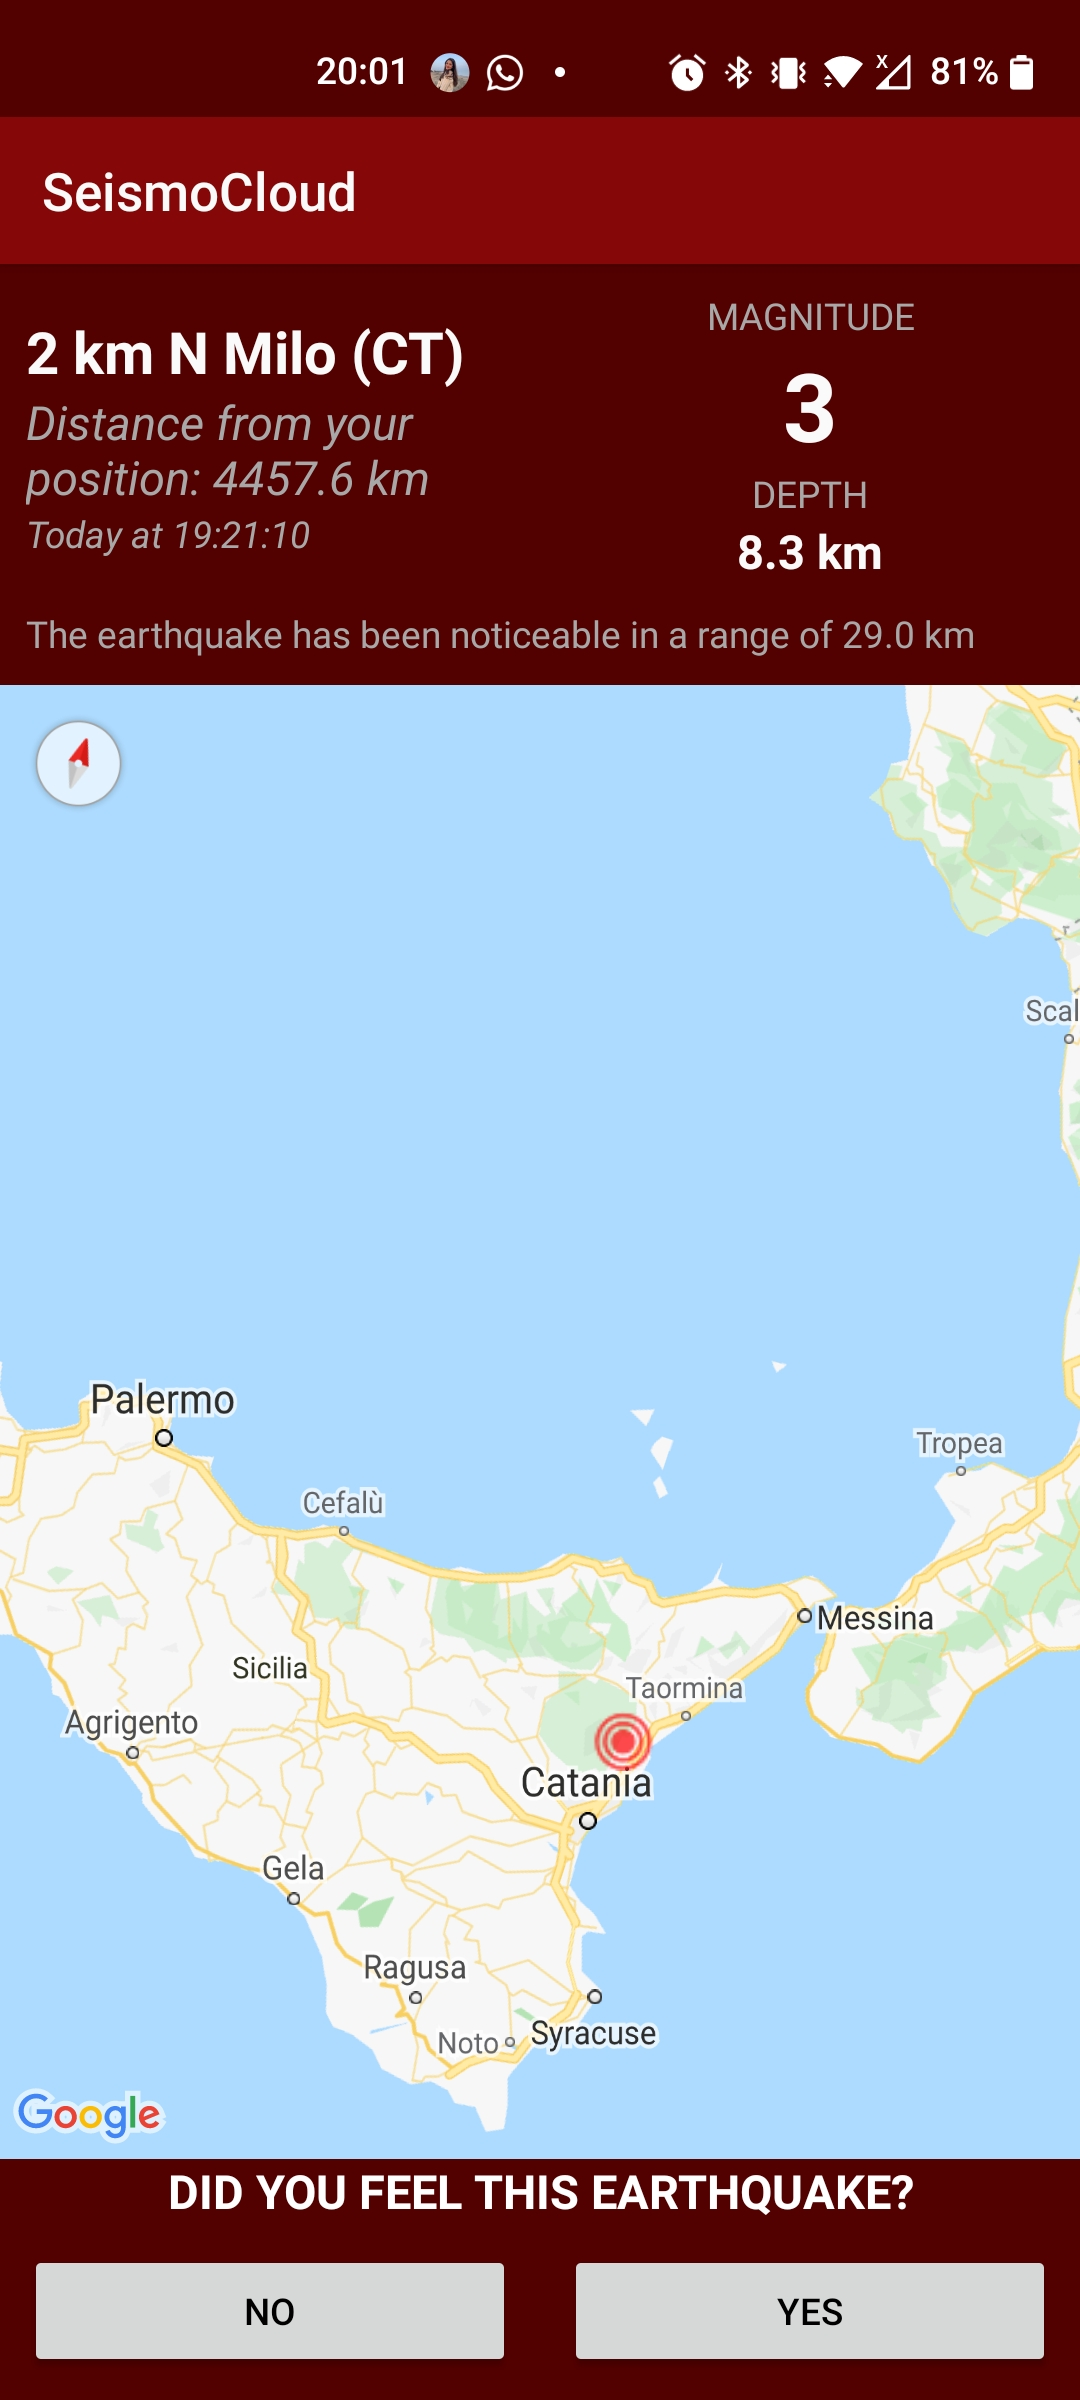
\includegraphics[width=0.9\linewidth]{images/applicationsurvey.png}
\caption{Schermata relativa ad un terremoto}
\label{fig:applicationsurvey}
\end{subfigure}

\caption{Schermate dell'applicazione SeismoCloud}
\label{fig:schermate}
\end{figure}

\section{Organizzazione del workflow}

Parte fondamentale del tirocinio è stata partecipare attivamente al progetto assieme ad altri tirocinanti e colleghi, con riunioni settimanali programmate per discutere il lavoro svolto nel time frame settimanale precedente, per chiarire dubbi su problemi incontrati e per confrontarsi. Un aspetto cruciale che ha permesso la cooperazione fin dal primo istante è stato utilizzare lo strumento di Version Control \textbf{Git} \cite{git}. Grazie ad esso, è possibile utilizzare uno speciale meccanismo di "checkpoint", i \textit{Commit}, che permettono il salvataggio del lavoro svolto sulla repository del progetto; l'utilità straordinaria è la possibilità di tornare ad uno stato precedente del progetto ed effettuare cambiamenti su versioni diverse del codice, non necessariamente secondo un ordine cronologico di cambiamenti. Ciò permette di ritornare sui propri passi nel caso in cui il codice modificato rispetto ad un \textit{Commit} precedente non permetta al sistema di funzionare correttamente. Se si ha l'urgenza di riportare il sistema ad una versione stabile, questa funzionalità appare ancora più funzionale.\\
Un secondo aspetto importante vede protagonisti i \textit{Branch}. Un \textit{Branch} rappresenta la linea temporale demarcata dai \textit{Commit} effettuati sul \textit{Branch} stesso. Possono essere creati moltissimi \textit{Branch}, ed è buona pratica seguire questa condotta: è sempre bene creare un \textit{Branch} per ogni nuova funzionalità che si sta implementando, per ogni \textit{hotfix} necessario a ripristinare il corretto funzionamento di una componente e per molti altri scenari.\\
Durante tutto lo svolgimento del tirocinio è stato necessario lavorare su uno o più \textit{Branch}, sia per non andare ad intaccare l'applicazione sottostante con dei cambiamenti e delle problematiche inevitabilmente introdotte nel corso dell'implementazione, sia per non entrare in conflitto con altri membri del team, ad esempio nella scrittura concorrente sullo stesso file.\\
\textit{Git} conta innumerevoli funzioni e comportamenti per favorire un ambiente di sviluppo quanto più organizzato e gestito possibile; si rimanda alla documentazione ufficiale dei comandi per una versione approfondita \cite{git}. 

\chapter{Analisi del problema}

\epigraph{"There were 5 exabytes of information created between the dawn of civilization through 2003, but that much information is now created every 2 days."}{\textit{Eric Schmidt (Google), 2010}}

%delete justify
\begin{flushleft}
\end{flushleft}
Un problema particolarmente noto e più che mai attuale riguarda i dati. La mole di dati che è collezionata quotidianamente nel mondo è inverosimile. Come ogni applicazione, servizio o sistema, anche SeismoCloud è sommersa costantemente da essi. La quantità ricevuta, come si denoterà di seguito, necessita di una riorganizzazione nel modo in cui essi sono collezionati, di come sono fruiti e dell'utilità che essi possono fornire in ambito interno ed esterno.

\section{Una nuova architettura per la collezione dei dati} \label{previousarch}

Uno dei flussi più imponente di dati riguarda le informazioni inviate periodicamente dai sensori: essendo essi gli strumenti di rilevazione di terremoti, elementi quindi imprescindibili per il corretto funzionamento interno del sistema nella sua totalità, è sempre importante monitorare ed acquisire sia gli aspetti più immediati dal punto di vista logico (quindi eventi sismici rilevati, posizione geografica per attribuire a questi ultimi un luogo), sia aspetti di apparente importanza superficiale, che di superficiale, in una prospettiva temporale ampia, hanno poco. Alcuni esempi sono la temperatura del sismometro, il suo indirizzo IP e l'alimentazione.

\paragraph{La quantità di dati}
L'aspetto cruciale che permette di quantificare come imponente la quantità di dati registrata dai sensori è il periodo di trasmissione: ogni dato viene difatti spedito ogni 5 minuti. Considerando un time frame giornaliero di 24 ore, si ha che il numero di trasmissioni per sensore è pari a:
\begin{equation} \label{eq:dailytrans}
transmissions = \frac{timeFrame}{sendingInterval} 
= \frac{24 * 60\ minutes}{5\ minutes} 
= 288\ transmissions
\end{equation}
Si consideri, inoltre, che i dati inviati per trasmissione sono i seguenti:\\
temperature, rssi, publicip, localip, threshold, bssid, essid.
Si immagini dunque come ogni giorno ciascun sensore produca 288 valori di ognuno degli elementi di cui sopra, non considerando i segnali di liveness che essi inviano ogni di 14 minuti (dato che, nel calcolo precedente, è stato trascurato). Ad essi si aggiungano un timestamp, per tenere traccia del momento dell'invio dei dati, e l'ID dei Sismometri, e si giunge ad un numero di dati inviato quotidianamente pari a:
\begin{equation} \label{eq:dailyoneseismo}
\begin{split}
dataSent = transmissions * len(elements) = \\
= 288\ transmissions * 9\ elements = 2592\ single\ elements\ sent
\end{split}
\end{equation}
dove, per \textit{len(elements)}, si intende il numero di elementi inviati dai sensori, quindi sommando singolarmente i dati quali temperature, rssi, ecc.\\
Come ultimo calcolo dimostrativo, si prenda come ipotesi che il numero di device attivi siano 100 (dato che rispecchia il numero attualmente attivo di device). Con una semplicissima moltiplicazione, si ottiene che il numero di dati ricevuti \textbf{ogni giorno} da SeismoCloud sono pari a:
\begin{equation} \label{eq:overalldailytrans}
dailyData = singleSeismoData * activeSeismos = 2592 * 100 = 259.200\ elems
\end{equation}
Appare quindi chiara la necessità di inserire i dati ricevuti in un nuovo sistema a sé stante, \textit{scalabile} e \textit{data-oriented}.

\paragraph{Il sistema attuale}
L'architettura del sistema, in una versione ad alto livello è rappresentata nella Figura \ref{fig:datainsertionmaria}.
Il collezionamento dei dati si articola nei seguenti passi:
\begin{itemize}
    \item I sensori inviano dati tramite il protocollo MQTT (Message Queue Telemetry Transport) \cite{mqtt} al Broker MQTT.
    \item Il Broker comunica con un controller.
    \item Il controller inserisce i dati nel database MariaDB. 
    \item I dati sono salvati nel database.
\end{itemize}
Il problema principale individuato è il salvataggio dei dati:\\
in primo luogo, il controller comunica direttamente con il database, inserendo in modo sincrono i dati. Un cambiamento di database comporterebbe una modifica nel controller;
in secondo luogo, i dati sono inseriti in un database che non ha una particolare predisposizione ai dati che rappresentano serie temporali di elementi, come quelli in esame. 
\begin{figure}[h]
    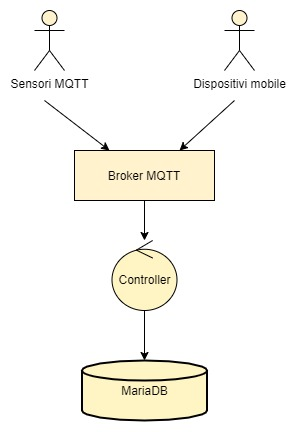
\includegraphics[scale=0.67, center]{images/insertdatamaria.jpg}   
    \caption{Architettura attuale per la gestione dei dati dei sensori.}
    \label{fig:datainsertionmaria}
\end{figure} 

\section{API per i dati storici} \label{apidatistorici}

\paragraph{Fornire dati agli utenti}
Le informazioni collezionate dai sensori sono disponibili solo internamente al sistema, o, eventualmente, su richiesta. Si vuole permettere ad utenti esperti di usufruirne per effettuare statistiche su di essi, indirizzarli al training di algoritmi di ML, o altre utilità che possano trovare.\\
Un accesso libero, tuttavia, non è assolutamente una soluzione ammissibile: permettere ad un utente (senza alcuna autenticazione) di richiedere \textbf{potenzialmente} ogni dato relativo ai sensori contenuto all'interno del database non solo gli permetterebbe di clonarli, manipolarli e distribuirli a suo piacimento, ma, come caso limite, porterebbe ad un possibile denial of service, in quanto impegnerebbe il server con una query con un risultato di dimensione notevole.\\
Un altro approccio considerato prevede la creazione di un set di API per soddisfare le richieste in modo controllato, ben delimitato nello span delle richieste possibili.
Quest'ultimo approccio è stato prediletto per l'esternazione dei dati.

\paragraph{Quali dati fornire ed entro quali limiti} 
Sulla base di quanto osservato in \ref{previousarch}, considerando inoltre il target principale delle API, si è scelto di fornire agli end user un subset delle informazioni inviate dai sensori, classificabili nelle due seguenti categorie:
\begin{itemize}
    \item Informazioni sullo status di alcune funzioni vitali del sensore
    \item Informazioni sulle scosse rilevate
\end{itemize}
In particolare, sul primo elemento si è stabilito di rendere disponibili dati quali la \textbf{Temperatura} del sismometro, il \textbf{RSSI} (Received Signal Strength Indication) ed il parametro di \textbf{Threshold}. \\
Per la maggior parte dei parametri l'importanza non risiede nel singolo valore degli stessi in un determinato istante di tempo, ma risultano estremamente più utili se analizzati in un periodo esteso. Un esempio lampante è l'analisi dei valori della temperatura del sensore in un periodo pari all'ultimo mese o anno, dati che potrebbero aiutare a prevenire un eventuale surriscaldamento prolungato (e conseguente rottura) di un dispositivo, permettendo al proprietario di installare un dispositivo di raffreddamento più adeguato o di programmarne lo spegnimento in determinate occasioni. Un discorso del tutto analogo può essere fatto per l'utilità degli altri dati.\\
Deve essere quindi possibile richiedere i dati specificando un range temporale.\\
In ultimo luogo, un criterio determinante per la selezione dei dati è per quali sensori effettuare la richiesta: ogni utente possiede l'identificativo dei propri sensori, per cui la richiesta dei relativi dati appare naturale.
Potrebbe essere però interessante (oltre che importante) richiedere i dati relativi ad una certa posizione geografica, estesa entro un certo raggio. Questa opzione, quindi, deve essere inclusa nella fase successiva di design.

\paragraph{Come fornire i dati}
Vista l'utilità che i dati dei Sismometri rappresentano, sarebbe piuttosto scomodo lato utente ricevere una risposta HTTP contenente tutti i risultati in formato \textbf{JSON} (JavaScript Object Notation) \cite{json}, come usualmente è effettuato in SeismoCloud per altri tipi di richieste: sarebbe invece più utile avere a disposizione i risultati all'interno di un file. Il formato del file in questione deve essere scelto in accordo con il suo possibile impiego: il formato \textbf{CSV} può essere particolarmente utile per consentire agli utenti di trasferire i dati ottenuti direttamente su fogli di calcolo, come \textbf{Excel} \cite{excel}, o per essere usati con librerie come \textbf{Pandas} \cite{pandas} per l'analisi dei dati. Un altro formato da rendere disponibile è il \textbf{GeoJSON} \cite{geojson}, formato di rappresentazione di oggetti geospaziali, con le loro proprietà e caratteristiche, basato su JSON. Ancora, un formato che potrebbe espandere l'utilizzo che si ha di questi dati è il \textbf{HDF5} \cite{hdf5}, usato, tra le altre cose, nel campo del Machine Learning (un esempio è la richiesta di utilizzare questo formato per il salvataggio di modelli \cite{tensorflow}). Infine, una ultima scelta da parte dell'utente può essere \textbf{MiniSeed} \cite{miniseed}, il cui acronimo sta per "mini Standard for the Exchange of Earthquake Data", per cui, per i dati relativi soprattutto alle scosse sismiche, sembra più che adatto. 

\section{Il tempo di una richiesta} \label{moledati}
Nella sezione \ref{apidatistorici} si è discusso circa i dati che il sistema dovrà fornire e le motivazioni principali legate all'utilizzo delle API. \\
Facendo riferimento ad un possibile Use Case di analisi statistica dei dati su un intervallo di anche solo un mese per un certo numero di Sismometri, è facile notare (facendo anche riferimento ai calcoli mostrati nell'equazione \ref{eq:dailyoneseismo} per un solo Sismometro) come la mole di informazioni da trasferire sia non indifferente.
Di fronte a queste cifre, ci si attende che il sistema non riesca ad elaborare ogni richiesta in maniera immediata, fornendo all'utente in modo sincrono tutti i dati richiesti. Una soluzione potrebbe essere ignorare la problematica e supporre che l'utente sia disposto ad attendere che la richiesta sia completata, ma ciò appare un modo di aggirare il problema piuttosto che risolverlo. Una soluzione più accurata prevede che la richiesta sia soddisfatta in modo \textbf{asincrono}, facendo in modo che l'utente possa effettuare una richiesta e poi essere libero di non attendere una risposta, mentre il sistema, internamente, la elabora. Le API devono essere quindi progettate per essere \textit{asincrone}: l'utente deve poter effettuare una richiesta ed essere in grado, una volta pronti i file, di ottenere i risultati. Deve quindi essere pensato sia un meccanismo di notifiche che notifichi l'utente nel momento in cui i risultati sono disponibili, sia un modo di accedere ai risultati stessi.

\paragraph{Back End ottimizzato}
Il fatto che si sia stabilito che le API siano asincrone non deve tuttavia rilassare i vincoli sul tempo di esecuzione di ogni richiesta: non ottimizzare il codice che verrà utilizzato per il Back End del sistema significa aumentare il tempo di risposta per un utente; inoltre, con poche accortezze, si rischia di sovraccaricare il server su cui il codice verrà installato con del lavoro inutile, portando a possibili failure dello stesso in caso di richieste a carico elevato o in caso di risorse non chiuse correttamente. Deve altresì essere possibile stabilire un tetto massimo di esecuzione, a livello temporale, per evitare di ricadere in richieste sottilmente volte all'estrazione di una quantità di dati spropositata, modellando in modo subdolo i parametri già discussi in \ref{apidatistorici}. 

\chapter{La soluzione - Design e Implementazione}

\section{Il linguaggio: Go}


\section{Il sistema Warehouse}

\subsection{Il sistema di code: NSQ}

\subsection{Il database: TimescaleDB}

\subsection{Il servizio di storage: MinIO}


\section{Realizzazione delle API}

In collaborazione con Gargano Daniele e Provornyy Igor sono state ideate e realizzate delle API per permettere agli utenti di ottenere i dati di cui alla sezione \ref{parametri}. Le API di seguito presentate sono le API su cui il lavoro che si sta mostrando si incentra maggiormente, per cui non saranno elencate e descritte le restanti.

\subsection{Il formato YAML}

\subsection{API byLocation}

\subsection{API byDevices}

\section{Processing delle richieste}

\subsection{Estrazione e Parsing}

La richiesta, in formato JSON, viene estratta da NSQ e "tradotto" in una struttura accuratamente ideata per rappresentare la richiesta.

\subsection{Interrogazione del database}

\subsection{Zip dei file}

\subsection{Upload su MinIO}

\chapter{Implementazione} \label{implementazione}
Avendo già definito il contesto in cui il \textit{WarehouseBackendWorker} andrà ad inserirsi, il lavoro che esso andrà a svolgere ed un primo abbozzo alle ottimizzazioni, una grande parte del lavoro può dirsi completata. Tuttavia, in fase di implementazione, sorgono molti problemi e conseguenti soluzioni, dovendo mettere in pratica ciò che si era trattato solo ad alto livello; è quindi necessario ragionare circa eventuali \textit{trade off}, approssimazioni eventuali, e, ovviamente, fare i conti con le limitazioni ed i punti di forza delle tecnologie che si stanno impiegando. In questo capitolo si introduce innanzitutto il linguaggio con cui il worker è stato realizzato, successivamente si mostrano le fasi di sviluppo del software che ne dà la vita, e, infine, si trattano alcune delle ottimizzazioni discusse precedentemente.
\section{Il linguaggio: Go}
Go \cite{go} (anche denominato \textit{Golang}) è un linguaggio Open Source compilato e staticamente tipizzato, pensato appositamente per essere semplice nella sintassi. Essa risulta difatti molto simile a quella del linguaggio C, mossa strutturale pensata appositamente per non rendere il passaggio tra un linguaggio ed un altro arduo. 
\begin{wrapfigure}{r}{0.25\textwidth}
\centering
    
\includegraphics{images/gopher.png}
    \caption{Gopher, la mascot di Go.}
    \label{fig:gopher}
\end{wrapfigure}
Go supporta l'uso di un \textit{Garbage Collector} (\textit{GC}) che ottimizza automaticamente l'uso della memoria, l'uso delle \textit{Reflection} per conoscere, ad esempio, il tipo delle variabili a run-time, e fornisce un meccanismo built-in per la concorrenza sotto forma di una metodologia a scambio di messaggi all'interno dei \textit{Canali}. Uno dei punti di forza, esterni alle caratteristiche intrinseche del linguaggio, risiede nella forza della comunità di sviluppatori che contribuiscono al miglioramento di Go; un esempio calzante dello spirito di comunità è chiaro se si pensa che il linguaggio ha addirittura una mascot (creata da Renee French), mostrata in Figura \ref{fig:gopher}. Proprio grazie a questo forte senso di comunità, la ridistribuzione del codice sorgente online per progetti, utilità e strumenti è particolarmente favorita. Per rendere disponibile il proprio codice ad altri sviluppatori, è fondamentale il concetto di \textbf{Moduli} e \textbf{Package}. In Go, un Modulo è un insieme di package, ed è propriamente l'elemento che uno sviluppatore può pubblicare e condividere. Un Package, invece, è un insieme di codice sorgente. Eventualmente, un Package può contenere altri Package.

\paragraph{Go in SeismoCloud} 
Nel progetto SeismoCloud, Go è utilizzato principalmente per la realizzazione delle API esposte all'utente, per alcuni worker che eseguono compiti specifici periodici (prendendo un esempio, la chiusura di una chat, lavoro dello studente Emanuele Petriglia \cite{emanuelepetriglia}) e per il \textit{WarehouseBackendWorker}, oltre ad altro codice sorgente di utilità per il lavoro.
In particolare, nell'ambito del Back End dell'applicazione SeismoCloud, il codice è contenuto all'interno di una repository e rappresentato da un modulo, con all'interno due package che svolgono compiti ben precisi: il package \textbf{cmd}, che contiene una serie di package rappresentanti i codici eseguibili, ed il package \textbf{service}, che rappresenta un singolo servizio per ogni package al suo interno. Contestualizzando quanto detto, in Figura \ref{fig:seismopackage} sono mostrati i package presentati.
\begin{figure}[h!]
    \centering
    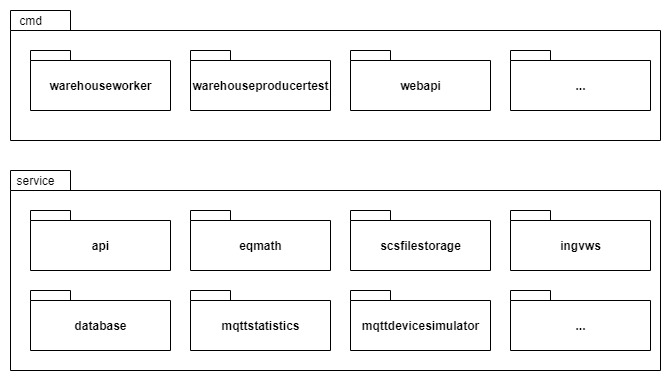
\includegraphics[width=\textwidth]{images/seismopackage.jpg}
    \caption{I package in SeismoCloud.}
    \label{fig:seismopackage}
\end{figure}
Uno dei package contenuto in \textbf{cmd}, e sviluppato per la realizzazione del codice eseguibile del \textit{WarehouseBackendWorker}, è \textbf{warehouseworker}: esso permette di rendere operativo il worker quando viene eseguito il codice. Invece, per citare un package in \textbf{service}, \textbf{eqmath} è un package che fornisce funzioni utili per alcuni calcoli relativi alla geometria spaziale, come il determinare se un punto (individuato da latitudine e longitudine) si trova all'interno di una data area geografica.\footnote{Questa funzione, nello specifico, è stata utilizzata nel corso dell'implementazione, per questo motivo è stata selezionata come esempio in questa sezione relativa alla correlazione tra Go e SeismoCloud.}

\section{Il WarehouseBackendWorker}
%definizione della struct Query e relativo code snippet
Nella sezione \ref{messageformat} si è mostrato il formato concordato per permettere una comunicazione unitaria tra Producer e Consumer di NSQ. Ovviamente, per poter essere utilizzato, il messaggio necessita di una mappatura 1-to-1 nei suoi campi con un elemento del linguaggio Go; un modo immediato di farlo è definire un \textbf{type} per la richiesta stessa, funzionalità permessa dal linguaggio di programmazione in questione. Il tipo scelto prende il nome di \textbf{Query} ed è una struct composta da tutti gli elementi definiti ed inseriti nel messaggio, per l'appunto. Il Codice Sorgente \ref{code:messageimpl} vuole essere sia un primo esempio dimostrativo di codice in Go, sia rappresentare il tipo Query stesso. 
\begin{listing}[h!]
\inputminted[baselinestretch=0.8]{go}{sources/query.go}
\caption{Il tipo Query.}
\label{code:messageimpl}
\end{listing}
Concentrandosi sul codice, si può notare come molti elementi siano di un tipo predefinito: \textbf{string}. Altri, come \textbf{Attributes}, sono tipi creati appositamente. I campi della struct Query non richiedono una spiegazione approfondita: essi rappresentano la loro controparte nel formato del messaggio, di cui si è già discusso in precedenza\footnote{Una nota importante, che permette di comprendere come lavori internamente il json decoder: il codice che presenta il pattern `json:"something"` è una caratteristica peculiare di Go, chiamata \textit{tag}. Con il tag, è possibile semplificare il lavoro del decoder indicandogli a quale chiave corrisponde nel JSON il campo in questione.}.

\paragraph{Il Consumer}
Creata una struttura per la rappresentazione del messaggio in Go, è ora necessario creare il Consumer. Propriamente, la creazione del consumer risulta abbastanza intuitiva, dovendogli solamente fornire (rimembrando il funzionamento di NSQ descritto in \ref{warehousedesign}) il nome del topic e del channel da cui riceverà i messaggi, oltre che un parametro di configurazione di NSQ. Bisogna poi registrare un \textit{Handler} che effettivamente svolga delle operazioni sul messaggio: senza alcun \textit{Handler}, il messaggio viene soltanto recapitato al Consumer, che non fa nulla. L'\textit{Handler} da registrare non è altro che un'interfaccia, denominata, per l'appunto, \textbf{Handler}. Questa interfaccia ha un solo metodo, la cui firma è:
\begin{minted}{go}
func HandleMessage(message *nsq.Message) error
\end{minted}
In Go, il concetto di interfaccia e di tipo che la implementa è abbastanza sottile: un tipo implementa implicitamente una interfaccia se esso implementa ogni metodo dell'interfaccia stessa. Per cui, per poter implementare l'interfaccia \textbf{Handler} e registrare un \textit{Handler} per la lavorazione dei messaggi, basta che una struttura implementi il metodo mostrato sopra. La struttura creata che lo implementa è il \textit{warehouseBackendWorker}, mostrata nel Codice Sorgente \ref{code:warehousebackendworker}.\footnote{In realtà, la situazione è leggermente più intricata, in quanto come Handler è registrata un'interfaccia ulteriore, che il warehouseBackendWorker implementa a sua volta. Questa situazione nasce da un discorso di visibilità dei tipi e per un corretto uso di alcune code practise, ma, ai fini di quanto trattato, è ininfluente.}
Si vuole far notare che, prima di raggiungere le versioni del codice presentato in tutto il capitolo, sono state necessarie diverse iterazioni che studiassero ed implementassero soluzioni sempre migliori. Questi raffinamenti possono essere approssimativamente inquadrati in tre fasi: 
\begin{itemize}
    \item Implementazione delle funzionalità principali.
    \item Implementazione della Streaming Pipe.
    \item Implementazione del Contesto della richiesta.
\end{itemize}
Lo scopo del capitolo non è confrontare in modo verboso i singoli cambiamenti tra le versioni, ma di dare un'idea del ragionamento alla base di essi e del perché sono stati introdotti. Per tale motivo verrà mostrato solamente il codice dell'ultima versione, e non i codici intermedi, ma se ne discuterà per evidenziarne le criticità, risolte poi dai suddetti cambiamenti. 

\begin{listing}
\inputminted[baselinestretch=0.8]{go}{sources/warehousebackendworker.go}
\caption{Il tipo warehouseBackendWorker.}
\label{code:warehousebackendworker}
\end{listing}

\section{Implementazione delle funzionalità}
I messaggi che vengono recapitati al Consumer sono elaborati dal worker, e, in particolare, dalla funzione \textit{HandleMessage}, riportata nel Codice Sorgente \ref{code:handlemessage}.
\begin{listing}
\inputminted[baselinestretch=0.9]{go}{sources/handlemessage.go}
\caption{La funzione che processa le richieste.}
\label{code:handlemessage}
\end{listing}
In esso sono trascurati alcuni elementi che coinvolgono i messaggi inseriti nel log e gli errori ritornati, tranne per la loro prima occorrenza: si vuole difatti evidenziare come il ruolo giocato dal log sia fondamentale per risalire ad eventuali errori o problemi nel corso del ciclo di vita del software e come il linguaggio consideri gli errori; essi sono gestiti esplicitamente, ed è buona pratica che una funzione abbia come tipo di ritorno un errore (che è un tipo built-in). La funzione è di per sé molto semplice: essa, difatti, demanda ogni compito del worker ad altre funzioni (si vedano \textit{GetResultsFromLocation} e \textit{SendNotification}). L'idea alla base è di identificare ogni compito delineato nella Figura \ref{fig:workerflow} con una funzione, in modo da modularizzare, ove possibile, il codice, rendendolo semplice, intuitivo e manutenibile, e rispettando sia i canoni dell'Ingegneria del Software, sia lo stile organizzativo del progetto. Una prima eccezione è l'estrazione e la consegna del messaggio, che vengono effettuate "automaticamente" secondo il meccanismo definito dal package NSQ, per cui non ha necessità di una funzione dedicata, così come la decodifica del messaggio, servizio offerto dalla libreria \textit{encoding/json}, e, in particolare, dalla funzione \textbf{json.Unmarshal}. 
\\
\\
Seguendo la pipeline delle istruzioni del worker, le funzioni \textit{GetResultsFromLocation} e \textit{GetResultsFromDevices} gestiscono le interrogazioni del Database, la scrittura dei file ed il caricamento su MinIO.\footnote{La dicitura "Location" al termine delle funzioni sviluppate sta ad indicare il soddisfacimento delle richieste che richiedono i dati non tramite Sismometri, ma tramite un'area geografica. Lo stesso discorso vale per "Devices". Questa distinzione è necessaria per alcune operazioni aggiuntive che devono essere effettuate nelle richieste con la dicitura Location, oltre che per favorire, ancora una volta, la semplicità e la modularità del codice. A livello pratico potrebbero essere accorpate nelle altre funzioni, ma minerebbero di molto questo stile di scrivere codice organizzato.} Prendendo come esempio \textit{GetResultsFromDevices} (Codice Sorgente \ref{code:getresults}), i passi che essa esegue per ogni attributo (ignorando la più volte chiamata \textit{CheckContextStatus}, di cui si parla in \ref{contesto}), in base agli attributi richiesti, sono:
\begin{enumerate}
    \item Chiamare una funzione Get\textit{Attributo}Query.
    \item Chiamare una funzione UploadQueryResultsByDevices.
\end{enumerate}
\begin{listing}[h!]
\inputminted[baselinestretch=0.8]{go}{sources/getresults.go}
\caption{La funzione che gestisce interrogazioni ed upload.}
\label{code:getresults}
\end{listing}
La prima effettua una query al Database relativa all'attributo di cui porta il nome, come \textbf{GetTemperatureQuery}. La seconda è una funzione che si occupa di effettuare la scrittura dei file e l'upload implicito su MinIO, dividendo i compiti in altre funzioni che scrivono ognuna un formato diverso di file (la funzione \textit{UploadCSVByLocation} si occupa dei file CSV ad esempio). Le funzioni che effettuano le query devono essere funzioni che assolvono solamente a tale scopo, per rispettare lo stile delle funzioni simili nel progetto.\\ \\
Le interrogazioni sono piuttosto semplici, per cui non ne verrà mostrato un esempio; è invece necessario concentrarsi su una qualsiasi delle funzioni per la scrittura dei file, come la già nominata \textit{UploadCSVByLocation}, riportata in breve nel Codice Sorgente \ref{code:uploadcsv}. L'aspetto saliente da notare ora è la \textbf{scrittura} del file all'interno del ciclo \textit{for}: si itera finché è presente un ulteriore risultato; ad ogni iterazione:
\begin{enumerate}
    \item Si inseriscono i dati della riga corrente di \textit{rows} in una struttura dati creata appositamente per contenerli.
    \item Si verifica che la posizione del sensore sia all'interno del raggio dell'area specificata nella richiesta. Si utilizza a tal proposito una funzione del package \textbf{eqmath} di SeismoCloud, ma i dettagli sono poco rilevanti in questo discorso.
    \item Il \textit{csvWriter}, una variabile di tipo puntatore a csv.Writer, scrive le informazioni presenti in \textit{csvLine} all'interno di \textit{fileInZipCSV}, un puntatore ad un file contenuto nell'archivio ZIP che si ottiene al termine del lavoro.
\end{enumerate}
Il meccanismo pensato specificamente per l'upload è discusso in \ref{streamingpipe}, dove apparirà chiaro il ruolo della variabile \textit{fileInZipCSV}.
\begin{listing}[h!]
\inputminted[baselinestretch=0.8]{go}{sources/uploadcsv.go}
\caption{La funzione che effettua la scrittura dei file e l'upload.}
\label{code:uploadcsv}
\end{listing}
Avanzando temporaneamente su questo aspetto, l'ultimo compito del worker riguarda il notificare l'utente che la richiesta è stata elaborata. Come già accennato, \textit{SendNotification} è la funzione preposta a fare ciò: essa chiama al suo interno funzioni diverse in base al metodo di invio della notifica scelto dall'utente. Una peculiarità delle funzioni di notifica implementate è che, nella gestione degli errori, qualsiasi errore è sempre inserito nel log ed ignorato, in quanto il lavoro è stato ultimato e non necessità di un'interruzione del flusso di esecuzione dei compiti. La notifica è una funzionalità extra offerta all'utente, che può comunque controllare lo status della propria richiesta tramite le API. La funzione è mostrata nel Codice Sorgente \ref{code:sendnotification}.
\begin{listing}[h!]
\inputminted[baselinestretch=0.8]{go}{sources/sendnotification.go}
\caption{La funzione che si occupa di inviare le notifiche.}
\label{code:sendnotification}
\end{listing}

\section{Implementazione della Streaming Pipe} \label{streamingpipe}
Nella precedente sezione si è mostrata la struttura ed il funzionamento generale del worker, posponendo però un passo importante: l'upload effettivo su MinIO. Inizialmente, esso era stato pensato in modo semplice, schematizzato nella Figura \ref{fig:salvataggiolocale}. Il problema che si sarebbe presentato una volta messo in funzione il sistema avrebbe però riguardato i file, che, esaudita una richiesta, sarebbero rimasti nello storage del server finché un'entità (fisica o digitale) non li avesse rimossi. Progettare un ulteriore worker che ripulisse lo spazio da file obsoleti non sembrava una via praticabile, tantomeno la migliore.
\begin{figure}[h!]
    \centering
    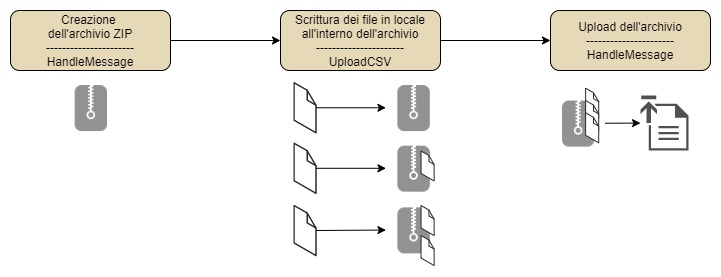
\includegraphics[width=\textwidth]{images/salvataggiolocale.jpg}
    \caption{Upload dei risultati con salvataggio locale}
    \label{fig:salvataggiolocale}
\end{figure}
Una versione aggiornata prevedeva la creazione di file temporanei, di cui il sistema operativo avrebbe gestito autonomamente l'eliminazione. Sembra una soluzione altamente più accettabile, ma le problematiche che continuano a presentarsi sono due: 
\begin{itemize}
    \item Il worker deve comunque scrivere sul disco, che si traduce in spendere maggiore tempo per ogni richiesta (si pensi, in caso di HDD, al tempo di accesso al disco, di rotazione, di ricerca, ecc.).
    \item Il worker esegue i propri compiti linearmente: crea innanzitutto l'archivio ZIP; finché non termina la scrittura di ciascuno dei file, il file ZIP non viene chiuso (allegando un file che funge da una sorta di indice con informazioni sui file presenti al suo interno). Per cui, i compiti sono eseguiti in ordine, con ogni step che deve attendere quello precedente per essere iniziato. In altre parole, l'upload deve attendere finché l'ultima riga dell'ultimo file è scritta. 
\end{itemize}
Si è pensato ad una soluzione che riuscisse a risolvere entrambe le problematiche. In particolare, per evitare l'accesso al disco si potrebbe pensare di memorizzare ogni dato scritto in memoria RAM; il problema evidente è la pericolosità di mantenere tutti i dati scritti in memoria, considerando la mole che ne deriverebbe da ogni richiesta: sebbene sia possibile aggregare e configurare memorie per estenderne la capacità totale, è sbagliato cercare un'ottimizzazione che sembra aggirare il problema invece che risolverlo, basandosi essa solamente sull'aumentare la memoria a disposizione. Se, tuttavia, i dati fossero scritti in modo progressivo mentre sono consumati altrettanto progressivamente, la memoria principale non si troverebbe sommersa di tutta la quantità dei dati scritti, ma di volta in volta di una certa frazione di essi. Dovrebbe essere creato un buffer che gestisce in automatico la sua dimensione, accettando dati in ingresso (la scrittura dell'archivio ZIP) e svuotandosi (upload su MinIO di porzioni dell'archivio) automaticamente. Il buffer non necessiterebbe di scrivere sul disco, ma rimarrebbe in memoria senza sovraccaricarla. L'idea è rappresentata in Figura \ref{fig:pipe}. 
\begin{figure}[h!]
    \centering
    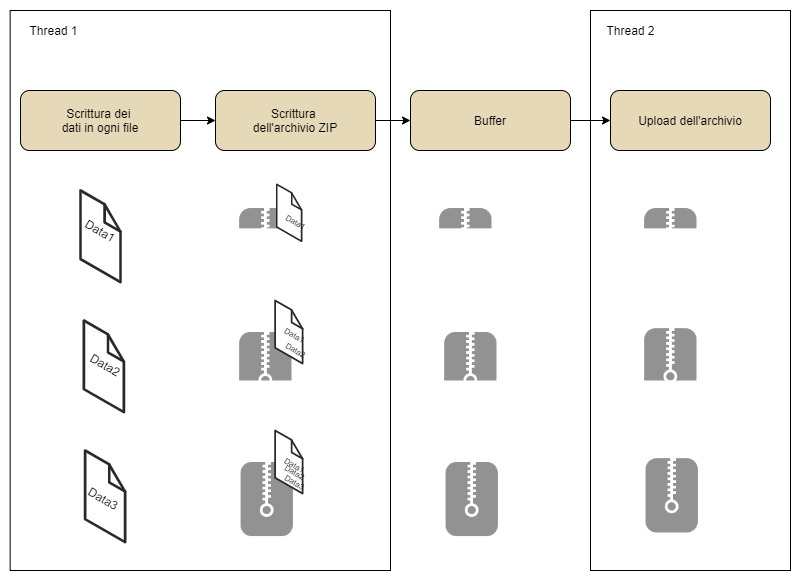
\includegraphics[width=\textwidth]{images/pipe.jpg}
    \caption{Sistema asincrono in memoria per la scrittura e l'upload.}
    \label{fig:pipe}
\end{figure}\\
Dal punto di vista implementativo, una funzione che il linguaggio Go mette a disposizione è \textbf{Pipe()}, del package \textit{io}. Essa crea una pipe in memoria, di cui permette la gestione in scrittura e lettura con i rispettivi valori di ritorno: \textit{PipeWriter} e \textit{PipeReader}. Le due estremità della pipe sono collegate direttamente; non esiste un buffering interno tra loro. Come si può vedere nel Codice Sorgente \ref{code:getresults}, la pipe è creata con l'istruzione:
\begin{minted}{go}
pipeReader,pipeWriter := io.Pipe()
\end{minted}
L'estremità di scrittura pipeWriter è collegata con \textit{writer}, uno zip.Writer che si occupa di scrivere l'archivio ZIP, tramite l'istruzione 
\begin{minted}{go}
writer := zip.NewWriter(pipeWriter)
\end{minted}
Questo comando specifica che l'archivio deve essere scritto \textbf{direttamente} all'interno della pipe, non toccando il disco.
Qualche riga di codice più avanti, invece, si delega ad una goroutine\footnote{Una goroutine è un thread gestito direttamente da Go che viene eseguito in parallelo rispetto al thread principale} l'upload su MinIO, collegando il lato reader della pipe all'interno della funzione preposta al caricamento:
\begin{minted}{go}
worker.fs.PutWarehouseResults(..., pipeReader, ...)
\end{minted}
Questa funzione effettua una serie di HTTP PUT verso il sistema di storage, elemento fondamentale per permettere un caricamento progressivo dei dati su di esso.
La variabile \textit{writer} viene poi passata in input a \textit{UploadQueryResultsByDevices}, che si collega alla funzione:
\begin{minted}{go}
func UploadCSVByLocation(userRequest Query,rows pgx.Rows,
zipWriter*zip.Writer,fileNamestring) error
\end{minted}
mostrata nel Codice Sorgente \ref{code:uploadcsv}. Si era detto che l'utilità della variabile \textit{fileInZipCSV} sarebbe stata chiarificata successivamente: ebbene, essa rappresenta un file che lo zip.Writer, creato in precedenza e passato in input, origina. In questo modo, i dati scritti ad ogni iterazione del ciclo \textit{for rows.Next()} sono inviati lungo questa catena di writer, fino a giungere alla goroutine, che continuerà a ricevere i dati di volta in volta, effettuando un upload progressivo. Questo sistema è stato chiamato \textit{Streaming Pipe}.

\section{Implementazione del Contesto} \label{contesto}
Allo stato descritto fin'ora, il sistema, in casi eccezionali, potrebbe andare in stallo e non terminare su una data richiesta; il rischio è che, per qualche problema, esso continui ad eseguire operazioni pesanti dal punto di vista dell'intero sistema, come la scrittura o il caricamento dei file. Un comportamento del genere non gestito, ovvero terminato, porterebbe ad un possibile collasso del server su cui il codice è installato. Qui entra in gioco il \textbf{Contesto} di una richiesta: le richieste devono avere un tempo massimo di esecuzione, superato il quale qualsiasi compito si stia svolgendo deve essere terminato. In Go è stato introdotto (in versioni precedenti del linguaggio) un package, \textbf{Context}, che fornisce tipi e funzioni utili ad interrompere un'azione dopo un certo ammontare di tempo. Il tipo fondamentale è chiamato proprio \textit{Context}, che contiene dei campi per verificare la deadline del contesto e gli errori relativi alla chiusura dello stesso per una cancellazione stabilita in precedenza o per lo scadere del tempo massimo. Per impostare un timeout al contesto, è sufficiente chiamare la funzione \textit{context.WithTimeout} con un tempo massimo indicato in input. Essendo parte integrante della \textit{standard library} del linguaggio, molti dei package che forniscono utilità importanti hanno introdotto l'estensione per supportare il tipo Context, compresi alcuni di quelli impiegati nello sviluppo del worker, tra cui il package \textbf{pgx}, per la comunicazione con TimescaleDB, e \textbf{minio-go}, per la comunicazione con MinIO. Nel Codice Sorgente \ref{code:handlemessage} sono presenti delle istruzioni per l'istanziazione del contesto e la sua eliminazione una volta terminato l'handling del messaggio attuale:
\begin{minted}{go}
ctx, cancel := context.WithTimeout(context.Background(), worker.deadline)
defer cancel()
\end{minted}
Il tempo di timeout della richiesta è configurabile dall'esterno tramite la variabile \textit{worker.deadline}, mentre la cancellazione avviene tramite la funzione cancel(). Una delle particolarità di Go è la possibilità di ritornare in output una funzione, come per la cancel(). Essa viene poi "rimandata" con la keywork \textit{defer}, che ritarda le istruzioni seguenti al termine della funzione in cui essa si trova. Creato il contesto, esso deve essere inserito in input in pressoché tutte le funzioni che lo supportano, cosicché un lavoro non ancora terminato dopo un ragionevole intervallo temporale possa essere soppresso. Questo è il caso di tutte le interrogazioni, della connessione a MinIO per l'upload, e delle varie scritture dei file. Per verificare lo stato del timeout del contesto, bisogna effettuare un check con \textit{ctx.Err()}, una funzione che ritorna l'errore interno del contesto, se presente. La funzione \textit{CheckContextStatus(ctx)} esegue semplicemente un controllo sulla tipologia di errore ritornato dal contesto. In caso di errore, esso viene ritornato, interrompendo la pipeline di istruzioni del worker, come si può notare nel Codice Sorgente \ref{code:getresults}. Come ultimo aspetto da mostrare nell'implementazione del contesto, la cancellazione del contesto entra in conflitto con l'aspetto asincrono della goroutine della \textit{Streaming Pipe}: nel caso in cui il thread principale (il thread che esegue \textit{HandleMessage}) terminasse prima della goroutine, la richiesta verrebbe cancellata (per la funzione posticipata cancel()) e la comunicazione ritornerebbe un errore. Risulta quindi necessario un meccanismo di sincronizzazione tra i thread. Essendo Go un linguaggio progettato per risolvere questo tipo di situazioni in modo semplice ed elegante, sono messi a disposizione diversi meccanismi per la concorrenza. Si è scelto di impiegare un \textbf{WaitGroup}, una struttura implementata sopra dei mutex. Essa permette di incrementare un \textbf{contatore} rappresentante i \textbf{lavori in esecuzione}, di decrementarlo al termine di ciascun lavoro e di bloccare l'esecuzione di una funzione finché tale valore non raggiunga lo zero. Nel codice implementato, il thread principale si blocca dopo aver terminato la scrittura dei file, quindi quando il lato Writer della pipe ha terminato il suo lavoro. Il blocco è dovuto all'aggiunta di un lavoro (la goroutine che effettua l'upload) alla WaitGroup. Terminando, la goroutine decrementa il contatore della WaitGroup. Il thread principale, che nel frattempo attende controllandolo, verifica che il valore sia effettivamente 0, e continua con il proprio lavoro. Questo permette una sincronizzazione tra i thread eseguiti concorrentemente.

\chapter{Conclusione e sviluppi futuri}


\chapter{Ringraziamenti}
Ho pensato spesso a cosa avrei scritto in questa sezione, cosa mi avrebbero suggerito il cuore e la mente in questo momento, quale dei due avrei seguito con maggior fedeltà. \\ \\ 
Non posso dire che questi tre anni siano stati semplici, per molti motivi. La facoltà che ho scelto mi ha sicuramente posto davanti a sfide sempre maggiori, che sono sempre riuscito ad affrontare, mettendomi in dubbio, spesso, cercando di migliorare, sempre, per passione e caparbietà. L'informatica è sempre stata un punto cardine per me, un mondo che ha sempre e sempre susciterà il mio interesse, che sarà sempre affascinante ed ineguagliabile. Lo capisco mentre ne parlo con chi ne sa di meno, con chi ne sa di più. \\ \\ 
Il tempo ha fatto il suo corso, imprescindibile, portando con sé persone a me care. Penso ai miei nonni, a mio zio, andati via in così poco tempo, così velocemente. Per non parlare della situazione nel mondo, della pandemia, delle quarantene: è come se una parte dell'esistenza fosse stata messa in pausa, come se la vita di molti di noi fosse stata messa in pausa. O, perlomeno, la mia. \\ \\ 
All'improvviso, però, in un momento irrintracciabile del tempo, esso torna a fluire. Il passato non sembra altro che passato, il futuro qualcosa di incerto da scrivere, il presente il momento in cui si vive. E, così, guardando indietro verso questi tre anni appena trascorsi, tutto assume un connotato nostalgico, una visione diversa di ciò che è stata. E ripenso a tutte le cose che invece sono state semplici, alle persone che li hanno resi indimenticabili, irrinunciabili. \\ \\ 
Voglio, a tal proposito, ringraziare innanzitutto il mio relatore, il prof. Emanuele Panizzi, cha ha contribuito alla formazione della mia passione per questo mondo con il corso che ho potuto seguire prima, con il tirocinio proposto poi. Rimanendo in questo contesto, voglio anche ringraziare il dottorando Enrico Bassetti, per essere stato sempre a disposizione per ogni dubbio, per avermi spinto a voler imparare sempre di più e per avermi insegnato moltissimo.
\\ \\ \\ \\
Voglio ringraziare la persona che mi ha sempre supportato, condiviso ogni ricordo, ogni momento, ogni situazione piacevole e spiacevole, Chiara. Non ho parole per descriverti. Sei sempre la mia forza interiore, il motivo per cui non posso mai darmi per vinto, e spero di ripagarti almeno in parte per tutto ciò che sei per me. A volte ti guardo pensando a come riesci ad essere così speciale, così unica. E penso che un grande merito va alla tua famiglia, che ringrazio per essere un punto di riferimento costante per me.\\ \\ 
Ringrazio la mia famiglia, papà per quei momenti padre e figlio non troppo convenzionali, come le "lezioni" su come progettare un impianto elettrico domestico, mamma per quell'ottimismo e quei sogni che, implicitamente, mi hanno sempre spinto a pensare in grande, a guardarmi intorno, ed i miei fratelli, che mi hanno insegnato tanto ed i cui consigli porterò sempre con me; penso alle conversazioni mai banali con Simone, alle sempre nuove idee di Alessandro, ai consigli paterni di Francesco, alle tante cose che ho da imparare anche da Leonardo, il più piccolo di noi; penso ai tanti nipoti(ni), alle nuore, alle cose belle che accadono, come la nascita di Federico, i momenti tutti assieme. \\ \\ 
Ringrazio i miei cugini, reali e "acquisiti" (Pami, Alessio, Stefano), nonna Anna, gli zii, i miei amici, a partire dai più stretti (è doveroso citare Giovanni, Filippo, Irene, Alessio, Giulia, Alessia, Alberto, Alice, Giuseppe, Eleonora, Mattia, Cassandra, Luigi) a quelli che non vedo più così spesso, a quelli che ho potuto conoscere solamente nell'ultimo anno dietro uno schermo. \\ \\ 
Ringrazio ogni persona che ho avuto il piacere di conoscere per quanto mi ha insegnato, per avermi fatto capire che c'è sempre qualcosa di nuovo da imparare, che è un po' il dogma di noi informatici. Ringrazio chi ha reso la mia vita più semplice o più difficile, perché non sempre le lezioni si imparano nel migliore dei modi. Ringrazio gli attimi da solo, i momenti di riflessione, il tempo trascorso da solo, perché non si può essere veramente felici se non si è felici con se stessi. E, infine, ringrazio chi mi ha insegnato che non sempre le cose vanno per il verso giusto; o che, a volte, il verso giusto non è rivolto verso di noi. E che, a volte, bisogna anche spostarsi per allinearsi ad esso.\\ \\
Tirando le somme del tempo trascorso non sempre è possibile essere grati per ciò che è stato: è più facile condannare il passato e rifugiarsi nel futuro piuttosto che accettarlo e rivalutarlo, cercando di ricordare cosa più di bello è stato.
Mi chiedo spesso se rifarei tutto ciò che ho fatto, se rivivrei tutto ciò che ho vissuto, se sceglierei ancora questo percorso che ho iniziato tre anni fa. Se tutto il sudore versato sarà mai ripagato. Se tutte le lezioni imparate saranno servite a qualcosa. \\ \\ La risposta è sempre sì. Finché posso contare su tutte queste fantastiche persone, la risposta sarà sempre sì.


\backmatter
\addcontentsline{toc}{chapter}{\protect\textbf{Elenco delle figure e codici sorgente}}
\addcontentsline{toc}{chapter}{\protect\textbf{Bibliografia}}

{\listoffigures \let\cleardoublepage\null \listoflistings}

\let\cleardoublepage\null

\printbibliography


\end{document}
